\documentclass[12pt]{article}

\setlength{\topmargin}{-.75in} \addtolength{\textheight}{2.00in}
\setlength{\oddsidemargin}{.00in} \addtolength{\textwidth}{.75in}

\usepackage{amsmath,color,graphicx,array,multirow,rotating, enumerate}
\usepackage{type1cm}
\usepackage{eso-pic}
\usepackage[hmargin=2cm,vmargin=1.3cm]{geometry}
\usepackage{mathabx}
\usepackage[rflt]{/Users/jgates/desktop/latex/floatflt}
\usepackage[table]{xcolor}
\nofiles

\def\Tab#1{\tabular[t]{>{\rule[-1ex]{0pt}{3ex}}c}#1\endtabular}
\newcolumntype{C}{@{}c@{}}

\pagestyle{empty}
\newcounter{ProbNum}
\setlength{\parindent}{0in}

% Watermark: graph paper
\newcommand\BackgroundPic{
\put(0,0){
\parbox[b][\paperheight]{\paperwidth}{%
\vfill
\centering

\includegraphics[width=\paperwidth,height=\paperheight,keepaspectratio]{/Users/jgates/desktop/latex/pics/plain.pdf}%
\vfill
}}}

%Diagram box command [v space][content]
\newcommand{\diagrambox}[2][40 mm]{
\framebox{\parbox{175 mm}{#2 \hfill \\ \vspace{#1}}}

\bigskip
}

% MakeList: [example number] [content]
\newcommand{\MakeList}[2]{
\begin{enumerate}[#1] \itemsep1pt \parskip0pt \parsep0pt  

#2
\end{enumerate}
}

\begin{document}



{\Large Problems tagged with standards:}CAPMG
\bigskip 
% Number 330
% CAPMG Units
% Graph conversion x->v->a
% JG

% Watermark
\AddToShipoutPicture*{\BackgroundPic}

\addtocounter {ProbNum} {1}

%\begin{floatingfigure}[r]{.3\textwidth}
%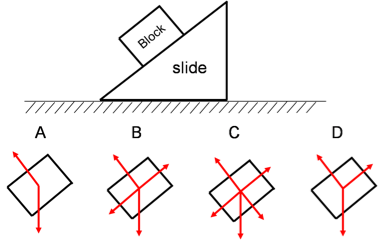
\includegraphics[scale=.4]{/Users/jgates/desktop/latex/pics/incline3.png}
%\end{floatingfigure}
 
{\bf \Large{330.}} Draw the velocity and acceleration graphs that correspond to the given position graph.

\begin{center}
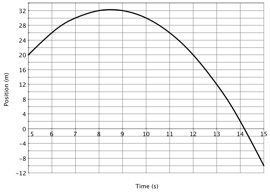
\includegraphics[scale=1]{/Users/jgates/desktop/latex/pics/givenxgraph1.png}
\end{center}

\begin{center}
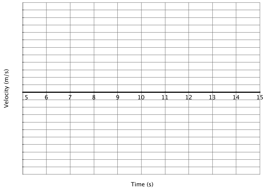
\includegraphics[scale=1]{/Users/jgates/desktop/latex/pics/blankvgraph1.png}
\end{center}

\begin{center}
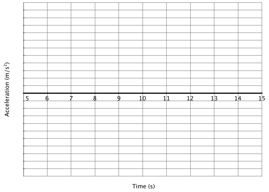
\includegraphics[scale=1]{/Users/jgates/desktop/latex/pics/blankagraph1.png}
\end{center}


\bigskip \vspace{6mm}% Number 340
% CAPMG Units
% Graph conversion a->v->x
% JG

% Watermark
\AddToShipoutPicture*{\BackgroundPic}

\addtocounter {ProbNum} {1}

%\begin{floatingfigure}[r]{.3\textwidth}
%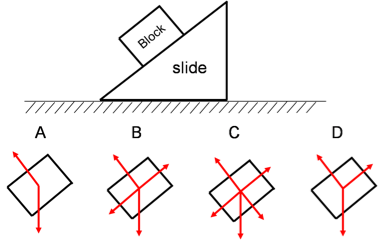
\includegraphics[scale=.4]{/Users/jgates/desktop/latex/pics/incline3.png}
%\end{floatingfigure}
 
{\bf \Large{340.}} Draw the position and velocity graphs that correspond to the given acceleration graph, initial position of -3 meters, and initial velocity of ${2~\tfrac{m}{s}}$.

\begin{center}
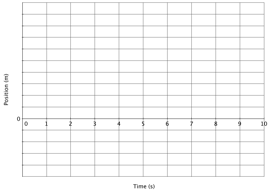
\includegraphics[scale=1]{/Users/jgates/desktop/latex/pics/blankxgraph2.png}
\end{center}

\begin{center}
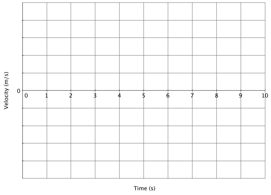
\includegraphics[scale=1]{/Users/jgates/desktop/latex/pics/blankvgraph2.png}
\end{center}

\begin{center}
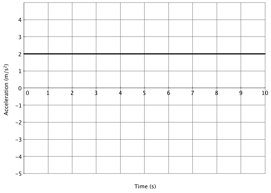
\includegraphics[scale=1]{/Users/jgates/desktop/latex/pics/givenagraph2.png}
\end{center}


\bigskip \vspace{6mm}% Number 360
% CAPMG 
% Token toss - qual graph stack describing motion, avg v
% JG

% Watermark
\AddToShipoutPicture*{\BackgroundPic}

\addtocounter {ProbNum} {1}

\begin{floatingfigure}[r]{.15\textwidth}
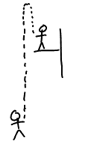
\includegraphics[scale=.8]{/Users/jgates/desktop/latex/pics/tokentoss.png}
\end{floatingfigure}
 
{\bf \Large{360.}} A man, on the ground, throws a subway token to his friend on the platform above.  The token is thrown essentially straight up; it flies past the friend and falls back to him. Call the lower man�s hand ${y=0}$ and define �up� as positive.

\bigskip  Draw graphs of the token�s vertical position, velocity, and acceleration during the trip.  No numbers are necessary.
Make sure that the time scales of the three graphs line up.

\begin{center}
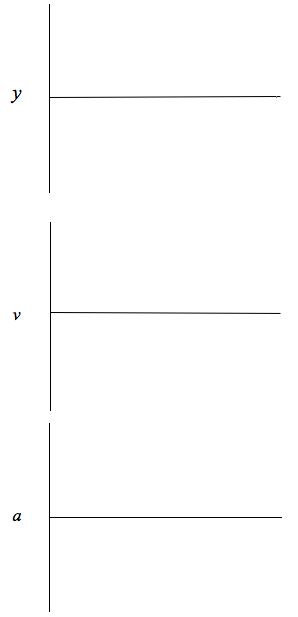
\includegraphics[scale=.85]{/Users/jgates/desktop/latex/pics/blankyvagraphstack.png}
\end{center}

\bigskip Finally, show on both the position and velocity graphs the \emph sign (is it positive, negative, or zero?) of the average velocity for the trip.  Be sure that it�s clear which characteristic of each graph you used to determine the sign of the average velocity!

\bigskip \vspace{6mm}% Number 371
% CAPMG Units
% Cannon shot straight up - how much time? Graphical
% JG

% Watermark
\AddToShipoutPicture*{\BackgroundPic}

\addtocounter {ProbNum} {1}

%\begin{floatingfigure}[r]{.15\textwidth}
%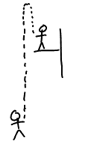
\includegraphics[scale=.8]{/Users/jgates/desktop/latex/pics/tokentoss.png}
%\end{floatingfigure}
 
{\bf \Large{371.}} A cannon is shot straight up into the air. The cannonball leaves the cannon moving ${45~\tfrac{m}{s}}$.  

\bigskip  After how much time in the air will it have a speed of ${20~\tfrac{m}{s}}$? Use graphical problem-solving.

%\begin{center}
%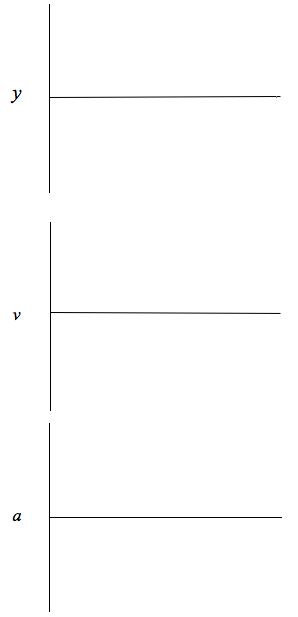
\includegraphics[scale=.85]{/Users/jgates/desktop/latex/pics/blankyvagraphstack.png}
%\end{center}


\bigskip \vspace{6mm}% Number 392
% CAPMG  Units
% Meteor chunk slowdown; algebraic version
% JG

% Watermark
\AddToShipoutPicture*{\BackgroundPic}

\addtocounter {ProbNum} {1}

%\begin{floatingfigure}[r]{.15\textwidth}
%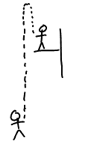
\includegraphics[scale=.8]{/Users/jgates/desktop/latex/pics/tokentoss.png}
%\end{floatingfigure}
 
{\bf \Large{392.}} A rock fragment is traveling ${640~\tfrac{m}{s}}$  when it is knocked off of a falling meteor. It has slowed to ${590~\tfrac{m}{s}}$  after .6 seconds.  Assume a constant acceleration. 

\bigskip
How far will it have gone after 2 seconds? Use graphical problem-solving.

%\begin{center}
%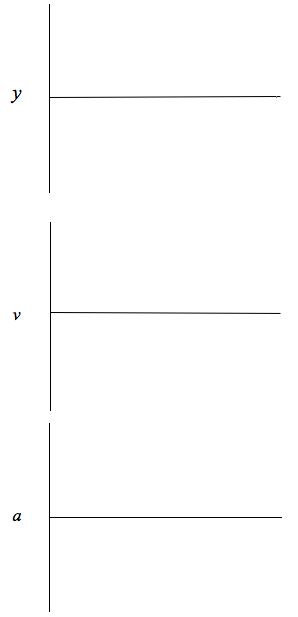
\includegraphics[scale=.85]{/Users/jgates/desktop/latex/pics/blankyvagraphstack.png}
%\end{center}


\bigskip \vspace{6mm}% Number 590
% UFPM  Inclines CAPMA CAPMG Algebra Units 
% Cart sliding up incline
% JG

% Watermark
\AddToShipoutPicture*{\BackgroundPic}

\addtocounter {ProbNum} {1}

%\begin{floatingfigure}[r]{.2\textwidth}
%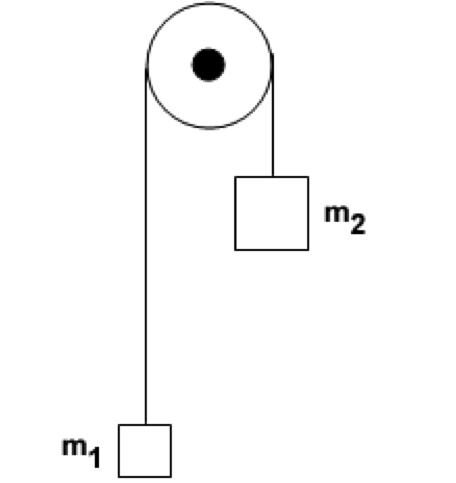
\includegraphics[scale=.8]{/Users/jgates/desktop/latex/pics/Atwood3}
%\end{floatingfigure}
 
{\bf \Large{590.}} A glider is given a quick push to start it moving up a ${7^{\circ}}$ inlined air track. The glider travels to a maximum distance of 112 cm up the track.

\bigskip
Determine the initial speed of the glider.
 
\bigskip \bigskip 
Draw a velocity graph for the glider; use the graph to determine how long the glider takes to get to that 112 cm point.
\bigskip 
Use your velocity graph to determine where the glider will be 2 seconds after it was launched.
\bigskip %\hfill 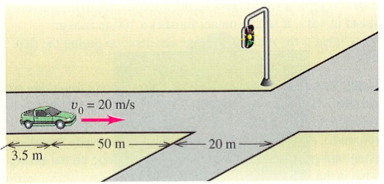
\includegraphics[scale=.85]{/Users/jgates/desktop/latex/pics/redlight.png}
\vspace{6mm}% Number 600
% CAPMA CAPMG Algebra Units 
% Overtaking - CAPM and CVPM
% JG

% Watermark
\AddToShipoutPicture*{\BackgroundPic}

\addtocounter {ProbNum} {1}

%\begin{floatingfigure}[r]{.2\textwidth}
%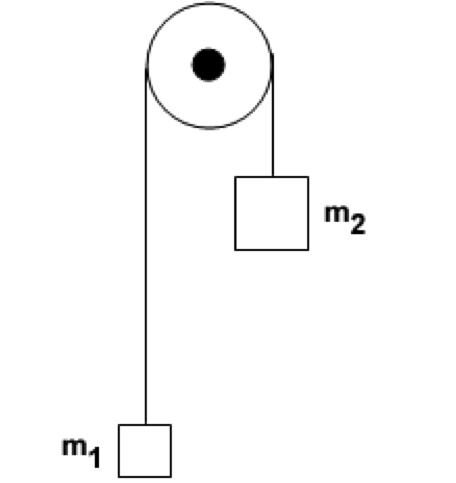
\includegraphics[scale=.8]{/Users/jgates/desktop/latex/pics/Atwood3}
%\end{floatingfigure}
 
{\bf \Large{600.}} A police car is driving towards a parked pair of criminals eating Zagnuts after pulling off a heist. The police car is moving ${40~\tfrac{m}{s}}$ and is initially .4 km away from the criminals. The criminals are going to drive away from the police car in an attempt to escape.  Assume that the crimemobile moves with a constant acceleration of ${1.8~\tfrac{m}{s^2}}$. 

\bigskip
Where will the police catch them?

\bigskip 
Draw a velocity graph for the criminals.  Use it to determine how far down they road they are when the police car passes their starting point.
\bigskip 
%\hfill 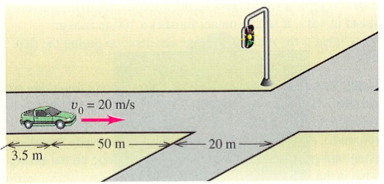
\includegraphics[scale=.85]{/Users/jgates/desktop/latex/pics/redlight.png}
\vspace{6mm}% Number 620
% UFPM CAPMG Algebra Units
% Graphs: F to a to delta v, varying F
% JG

% Watermark
\AddToShipoutPicture*{\BackgroundPic}

\addtocounter {ProbNum} {1}

\begin{floatingfigure}[r]{.54\textwidth}
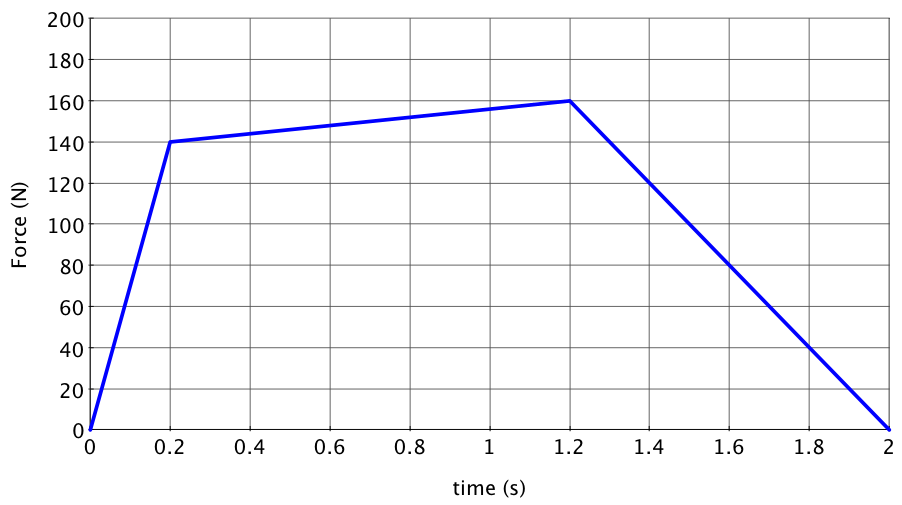
\includegraphics[scale=.7]{/Users/jgates/desktop/latex/pics/Fvst1}
\end{floatingfigure}
 
{\bf \Large{620.}} A 50 kg peewee football player runs into a stationary 40 kg player at an initial speed of 4 meters per second. The magnitude of the force exerted by the football players on each other is shown as a function of time. 

\bigskip
Draw quantitatively accurate acceleration graphs for each player.
\paragraph{}
\noindent
\bigskip Use your acceleration graphs to determine the players' final velocities.
\bigskip 
Draw a motion diagram showing the players' motions before and after the collision.
\bigskip 
%\hfill 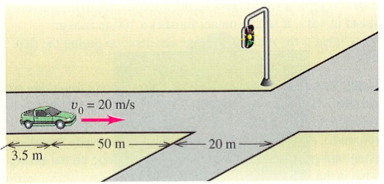
\includegraphics[scale=.85]{/Users/jgates/desktop/latex/pics/redlight.png}
\vspace{6mm}% Number 780
% CAPMA CAPMG Algebra Units 
% Rocket AP problem - graphical and algebraic
% Mostly AP/some JG

% Watermark
\AddToShipoutPicture*{\BackgroundPic}

\addtocounter {ProbNum} {1}

%\begin{floatingfigure}[r]{.44\textwidth}
%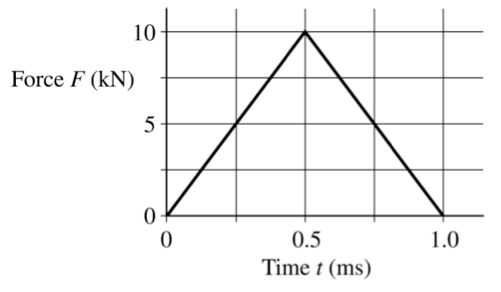
\includegraphics[scale=.5]{/Users/jgates/desktop/latex/pics/collisiongraph1}
%\end{floatingfigure}
 
{\bf \Large{780.}} A two stage rocket leaves its launch pad moving vertically with an average acceleration of ${4~\tfrac{m}{s^2}}$.  10 seconds after launch, the first stage of the rocket (now without fuel) separates from the second stage  The second stage now has an upward acceleration of ${6~\tfrac{m}{s^2}}$.  

\bigskip
How high is the rocket when the first stage separates?

\bigskip 
What will be the maximum height attained by the first stage after separation?

\bigskip 
\vspace{6mm}% Watermark
\AddToShipoutPicture*{\BackgroundPic}
Draw position, velocity, and acceleration graphs for the first and second stages' motions {\emph after separation} on the same three sets of axes (that is, have both velocity graph on one set of axes, both position graphs on another, etc.).

\bigskip 
\bigskip 
Use the graphs to determine how far apart the stages are 4 seconds after separation.

\bigskip %\hfill 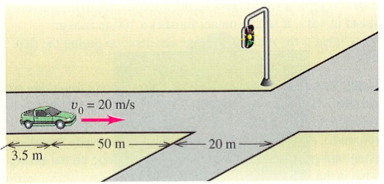
\includegraphics[scale=.85]{/Users/jgates/desktop/latex/pics/redlight.png}
\vspace{6mm}% Number 800
% CAPMG Units 
% x graph -find v, a
% JG

% Watermark
\AddToShipoutPicture*{\BackgroundPic}

\addtocounter {ProbNum} {1}

%\begin{floatingfigure}[r]{.44\textwidth}
%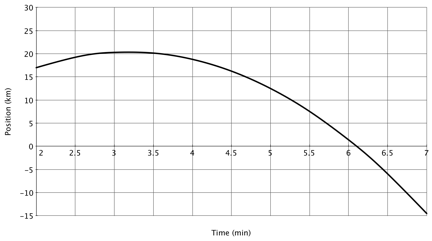
\includegraphics[scale=.5]{/Users/jgates/desktop/latex/pics/xgraph2}
%\end{floatingfigure}
 
{\bf \Large{800.}} Use the graph to determine the object's initial velocity and its acceleration, using graphical methods. Draw any additional graphs that you need for your solution below.\bigskip

\begin{center}
 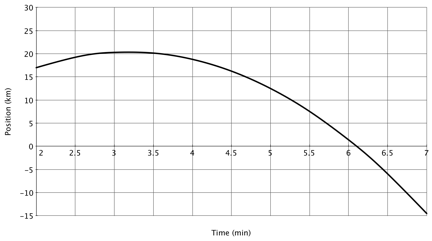
\includegraphics[scale=1]{/Users/jgates/desktop/latex/pics/xgraph2}
\end{center}

\bigskip \vspace{6mm}% Number 810
% CAPMG Units 
% Clay/Jax chase - graphical
% JG

% Watermark
\AddToShipoutPicture*{\BackgroundPic}

\addtocounter {ProbNum} {1}

%\begin{floatingfigure}[r]{.44\textwidth}
%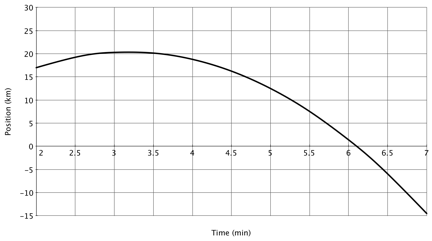
\includegraphics[scale=.5]{/Users/jgates/desktop/latex/pics/xgraph2}
%\end{floatingfigure}
 
{\bf \Large{810.}} Jax is sitting by the side of the road on his motorcycle when Clay zips by at 30 meters per second.  Jax immediately takes off in pursuit, driving with a constant acceleration.  Jax accelerates to Clay's speed within 15 seconds. \bigskip

How far behind Clay will Jax be at that moment that their speeds are equal?  Use graphical methods. \paragraph{}
\noindent

%\begin{center}
%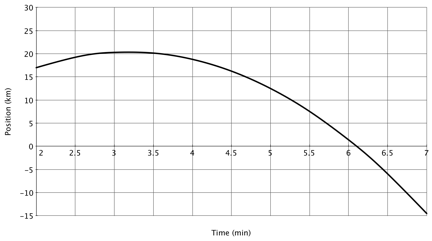
\includegraphics[scale=1]{/Users/jgates/desktop/latex/pics/xgraph2}
%\end{center}

\bigskip \vspace{6mm}% Number 813
% CAPMG  Units 
% Clay/Jax chase hard - graphical
% JG

% Watermark
\AddToShipoutPicture*{\BackgroundPic}

\addtocounter {ProbNum} {1}

%\begin{floatingfigure}[r]{.44\textwidth}
%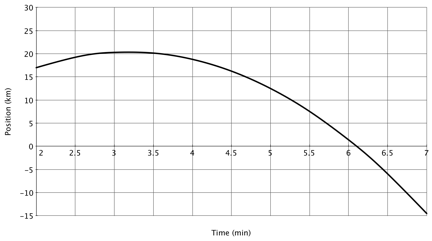
\includegraphics[scale=.5]{/Users/jgates/desktop/latex/pics/xgraph2}
%\end{floatingfigure}
 
{\bf \Large{813.}} Jax is sitting by the side of the road on his motorcycle when Clay zips by at 30 meters per second.  Jax immediately takes off in pursuit, driving with a constant acceleration.  Jax accelerates to Clay's speed within 15 seconds. \bigskip

How long will it take Jax to catch Clay?  Use graphical methods. \paragraph{}
\noindent

%\begin{center}
%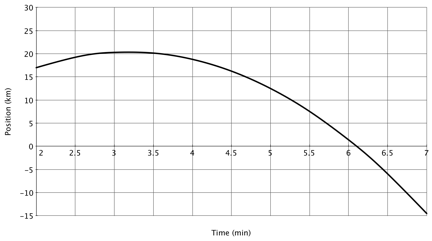
\includegraphics[scale=1]{/Users/jgates/desktop/latex/pics/xgraph2}
%\end{center}

\bigskip \vspace{6mm}% Number 821
% CAPMG Units 
% Rocket launch, freefall afterwards - difficult graphical
% JG

% Watermark
\AddToShipoutPicture*{\BackgroundPic}

\addtocounter {ProbNum} {1}

%\begin{floatingfigure}[r]{.44\textwidth}
%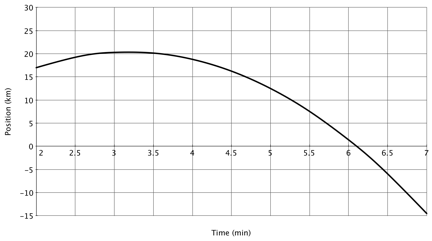
\includegraphics[scale=.5]{/Users/jgates/desktop/latex/pics/xgraph2}
%\end{floatingfigure}
 
{\bf \Large{821.}} A rocket blasts off, traveling with an acceleration of ${4~\tfrac{m}{s^2}}$ upward.  When it is 2000 meters above the ground, its engine shuts off. \bigskip

How much time was required for the rocket to reach the 2000 meter altitude, and how fast was it moving at that moment? Use graphical methods.\paragraph{}
\noindent

%\begin{center}
%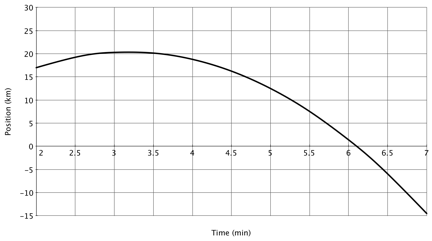
\includegraphics[scale=1]{/Users/jgates/desktop/latex/pics/xgraph2}
%\end{center}

\bigskip \vspace{6mm}% Number 861
% CAPMG Units 
% Car skidding to a stop graphical
% JG

% Watermark
\AddToShipoutPicture*{\BackgroundPic}

\addtocounter {ProbNum} {1}

%\begin{floatingfigure}[r]{.44\textwidth}
%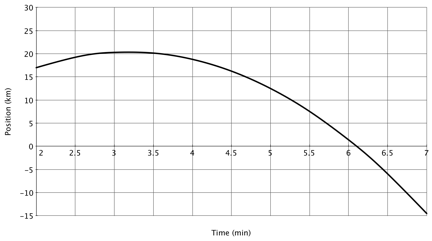
\includegraphics[scale=.5]{/Users/jgates/desktop/latex/pics/xgraph2}
%\end{floatingfigure}
 
{\bf \Large{861.}} A car traveling with a speed of 30 meters per second (a little more than 60 mph) slams on the brakes, coming to a stop after 5.2 seconds.   \bigskip

How far did the car travel during the slide?\paragraph{}
\noindent
\vfill


%\begin{center}
%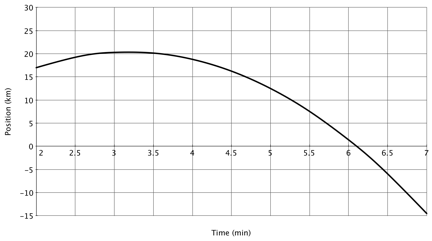
\includegraphics[scale=1]{/Users/jgates/desktop/latex/pics/xgraph2}
%\end{center}


\vspace{6mm}% Number 870
% CAPMG Units 
% Car skidding to a stop graphical
% JG

% Watermark
\AddToShipoutPicture*{\BackgroundPic}

\addtocounter {ProbNum} {1}

%\begin{floatingfigure}[r]{.44\textwidth}
%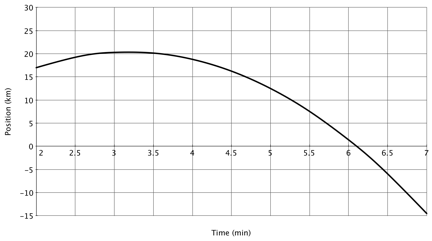
\includegraphics[scale=.5]{/Users/jgates/desktop/latex/pics/xgraph2}
%\end{floatingfigure}
 
{\bf \Large{870.}} A car traveling with a speed of 30 meters per second (a little more than 60 mph) slams on the brakes.  The wheels lock up and the tires skid on the road, providing an acceleration of magnitude ${11~\tfrac{m}{s^2}}$.   \bigskip

How far did the car travel during the slide? Use graphical methods.\paragraph{}
\noindent
\vfill


%\begin{center}
%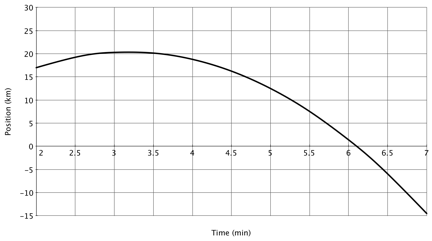
\includegraphics[scale=1]{/Users/jgates/desktop/latex/pics/xgraph2}
%\end{center}


\vspace{6mm}% Number 880
% CAPMG  Units 
% v graph problem-solving; v bar and displacement
% KO

% Watermark
\AddToShipoutPicture*{\BackgroundPic}

\addtocounter {ProbNum} {1}

\begin{floatingfigure}[r]{.44\textwidth}
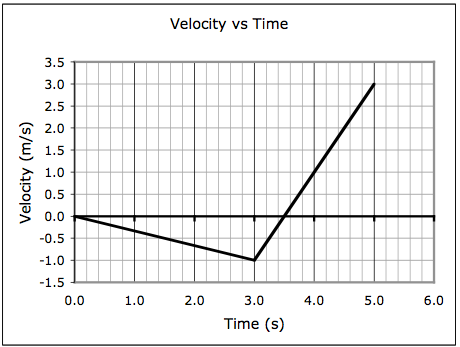
\includegraphics[scale=.54]{/Users/jgates/desktop/latex/pics/vgraph6}
\end{floatingfigure}
 
{\bf \Large{880.}} A cart travels with the velocity shown in the graph.   \bigskip


Describe the motion in words.
\paragraph{}
\noindent
\vfill

What is the cart's displacement, in meters, during the first four seconds?
\bigskip 
What was the cart's average velocity over the entire five seconds of recorded motion?
\bigskip 
At what instant does the cart reach the farthest position in the negative direction with respect to its starting point? (Explaining your thinking might help you get the right answer and will help me help you if you�re wrong.)
\bigskip 
%\begin{center}
%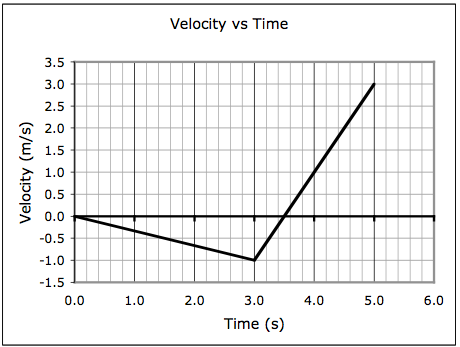
\includegraphics[scale=1]{/Users/jgates/desktop/latex/pics/vgraph6}
%\end{center}


\vspace{6mm}% Number 890
% CAPMG  Units 
% Graphs modeling motion
% KO

% Watermark
\AddToShipoutPicture*{\BackgroundPic}

\addtocounter {ProbNum} {1}

%\begin{floatingfigure}[r]{.44\textwidth}
%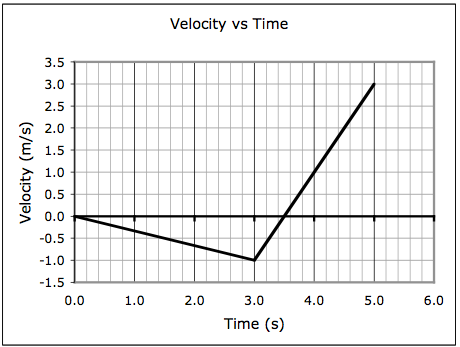
\includegraphics[scale=.54]{/Users/jgates/desktop/latex/pics/vgraph6}
%\end{floatingfigure}
 
{\bf \Large{890.}} For each of the following motions, draw a position graph and a velocity graph (with accurate numbers on the axes). Define up/right positive, down/left negative. As always, state any assumptions that you make.\bigskip

A car starts from rest, steadily speeds up to ${30~\tfrac{m}{s}}$ in 15 seconds, moves at a constant speed for 30 seconds, then comes to a halt in 5 seconds.
\bigskip 
A rock is dropped from a bridge and steadily speeds up as it falls. It is moving at ${30~\tfrac{m}{s}}$ three seconds later, when it hits the ground.

\bigskip %\begin{center}
%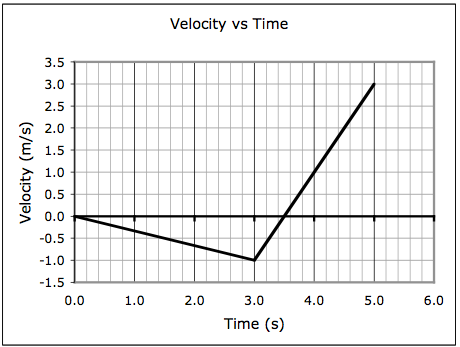
\includegraphics[scale=1]{/Users/jgates/desktop/latex/pics/vgraph6}
%\end{center}


\vspace{6mm}% Number 890
% CAPMG  Units 
% Graphs modeling motion
% JG

% Watermark
\AddToShipoutPicture*{\BackgroundPic}

\addtocounter {ProbNum} {1}

%\begin{floatingfigure}[r]{.44\textwidth}
%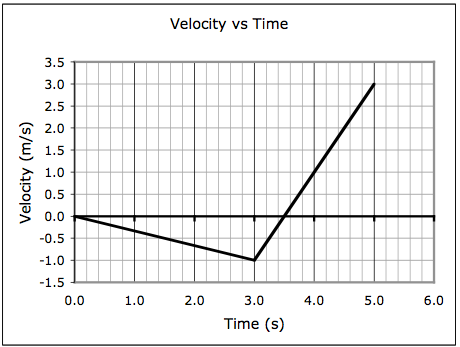
\includegraphics[scale=.54]{/Users/jgates/desktop/latex/pics/vgraph6}
%\end{floatingfigure}
 
{\bf \Large{900.}} For each of the following motions, draw a position graph and a velocity graph (with accurate numbers on the axes). Define up/right positive, down/left negative. As always, state any assumptions that you make.\bigskip

A car starts from rest, steadily speeds up to ${30~\tfrac{m}{s}}$ in 15 seconds, moves at a constant speed for 30 seconds, then comes to a halt in 5 seconds.
\bigskip 
A rock is dropped from a bridge and steadily speeds up as it falls. It is moving at ${30~\tfrac{m}{s}}$ three seconds later, when it hits the ground.

\bigskip 
%\begin{center}
%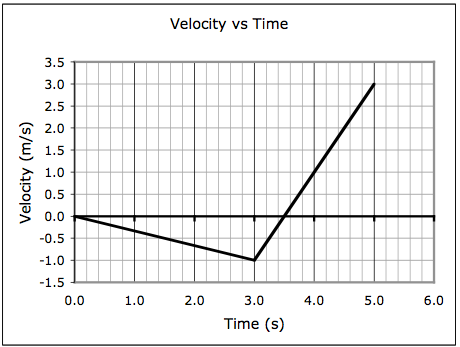
\includegraphics[scale=1]{/Users/jgates/desktop/latex/pics/vgraph6}
%\end{center}


\vspace{6mm}% Number 920
% CAPMG  Units 
% Rocket upwards - max. v, h?
% JG

% Watermark
\AddToShipoutPicture*{\BackgroundPic}

\addtocounter {ProbNum} {1}

%\begin{floatingfigure}[r]{.44\textwidth}
%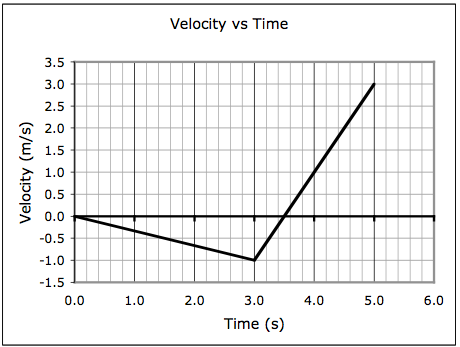
\includegraphics[scale=.54]{/Users/jgates/desktop/latex/pics/vgraph6}
%\end{floatingfigure}
 
{\bf \Large{920.}} A rocket launches and travels upwards with an acceleration of ${4.5~\tfrac{m}{s^2}}$ for 6 seconds; at that point it runs out of fuel and goes into freefall.   \bigskip

Determine the rocket's maximum speed on the upwards trip and maximum height using graphical methods.  \vfill


%\begin{center}
%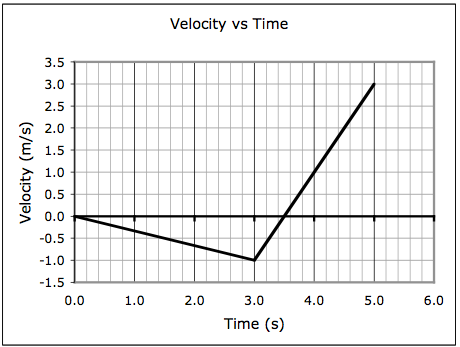
\includegraphics[scale=1]{/Users/jgates/desktop/latex/pics/vgraph6}
%\end{center}


\vspace{6mm}% Number 931
% CAPMG CVPMG  Units 
% Car driving - CAPM then CVPM, Graphical
% JG

% Watermark
\AddToShipoutPicture*{\BackgroundPic}

\addtocounter {ProbNum} {1}

%\begin{floatingfigure}[r]{.44\textwidth}
%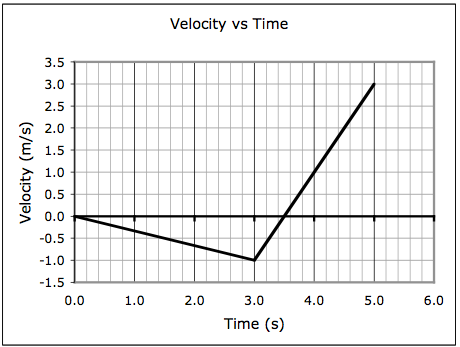
\includegraphics[scale=.54]{/Users/jgates/desktop/latex/pics/vgraph6}
%\end{floatingfigure}
 
{\bf \Large{931.}} A car accelerates from rest to ${25~\tfrac{m}{s}}$ in 4.3 seconds. It then maintains that speed for 10 seconds.    \bigskip

How far has it traveled during this motion?  Use graphical methods.\vfill


%\begin{center}
%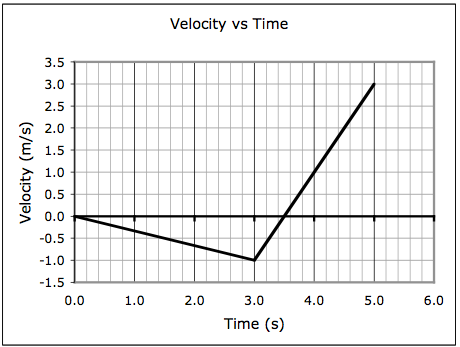
\includegraphics[scale=1]{/Users/jgates/desktop/latex/pics/vgraph6}
%\end{center}


\vspace{6mm}% Number 951
% CAPMG Units 
% Car slowing, a given - graphical
% JG

% Watermark
\AddToShipoutPicture*{\BackgroundPic}

\addtocounter {ProbNum} {1}

%\begin{floatingfigure}[r]{.44\textwidth}
%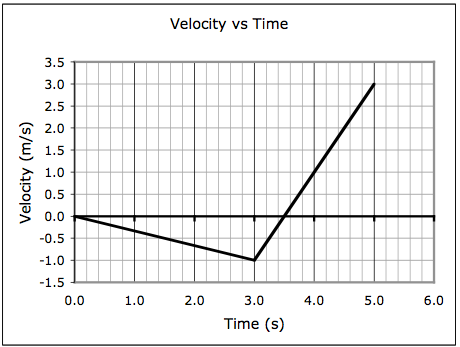
\includegraphics[scale=.54]{/Users/jgates/desktop/latex/pics/vgraph6}
%\end{floatingfigure}
 
{\bf \Large{951.}} A car drives down the road at ${18~\tfrac{m}{s}}$.  It slows down at a rate of ${2.2~\tfrac{m}{s}}$ per second.  \bigskip

After how much time will it be moving with a speed of ${7~\tfrac{m}{s}}$? Use graphical methods.
\bigskip 
How far did the car travel during the motion described above? Use graphical methods.
 \vfill


%\begin{center}
%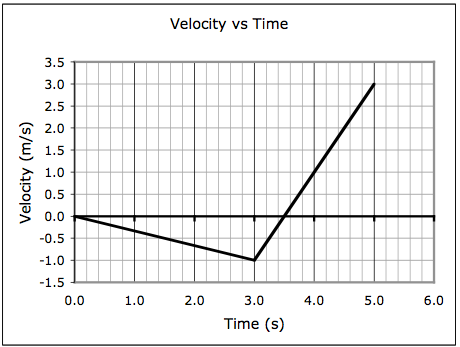
\includegraphics[scale=1]{/Users/jgates/desktop/latex/pics/vgraph6}
%\end{center}


\vspace{6mm}% Number 960
% CAPMG CVPMG Units 
% Drag racer - CAPM and CVPM - graphical
% JG

% Watermark
\AddToShipoutPicture*{\BackgroundPic}

\addtocounter {ProbNum} {1}

%\begin{floatingfigure}[r]{.44\textwidth}
%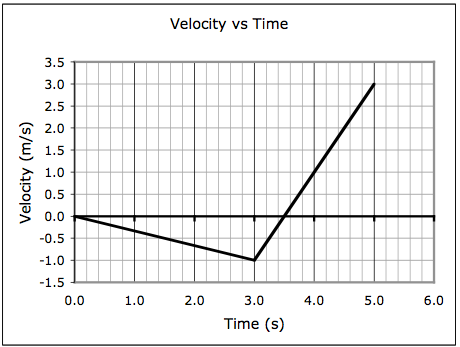
\includegraphics[scale=.54]{/Users/jgates/desktop/latex/pics/vgraph6}
%\end{floatingfigure}
 
{\bf \Large{960.}} A drag racer begins at rest, and accelerates to ${140~\tfrac{m}{s}}$ within 2.1 seconds.  Once at this speed, the racer maintains it through the finish line, which is 400 meters from the start line. \bigskip

Draw position, velocity, and acceleration graphs for this motion, with accurate values on all axes.  Make sure to denote the time at which the racer finishes the race.
\bigskip 

%\begin{center}
%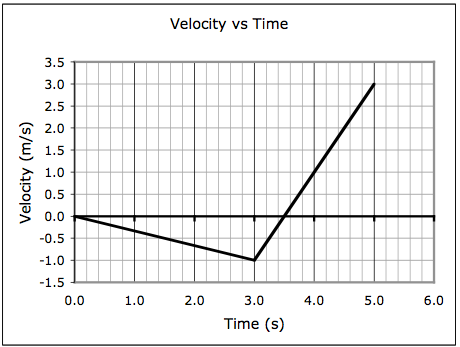
\includegraphics[scale=1]{/Users/jgates/desktop/latex/pics/vgraph6}
%\end{center}


\vspace{6mm}% Number 962
% CAPMG NAPM  Units 
% Drag racer - CAPM and CVPM, NAPM - graphical
% JG

% Watermark
\AddToShipoutPicture*{\BackgroundPic}

\addtocounter {ProbNum} {1}

%\begin{floatingfigure}[r]{.44\textwidth}
%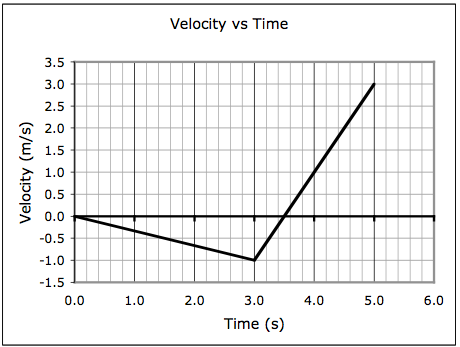
\includegraphics[scale=.54]{/Users/jgates/desktop/latex/pics/vgraph6}
%\end{floatingfigure}
 
{\bf \Large{962.}} A drag racer begins at rest, and accelerates to ${124~\tfrac{m}{s}}$.  Once at this speed, the racer maintains it through the finish line, which is 400 meters from the start line. The car deploys a parachute after crossing the finish line.  The magnitude of the acceleration provided by the air hitting the parachute is initially ${12~\tfrac{m}{s^2}}$.
\bigskip

Assuming that this acceleration is constant, how far will the car travel after crossing the finish line but before coming to a stop? Use graphical methods.
\bigskip 
The acceleration depends on the speed of the car, however: the magnitude of the acceleration decreases as the car slows down.  Incorporate this idea into your analysis and come up with a new estimate of the stopping distance.  Any reasonable model consistent with what I've told you is fine.
\bigskip %\begin{center}
%\includegraphics[scale=1]{/Users/jgates/desktop/latex/pics/vgraph6}
%\end{center}


\vspace{6mm}% Number 970
% CAPMG NAPM  Units 
% Changing v - graphical
% JG

% Watermark
\AddToShipoutPicture*{\BackgroundPic}

\addtocounter {ProbNum} {1}

\begin{floatingfigure}[r]{.44\textwidth}
\includegraphics[scale=.92]{/Users/jgates/desktop/latex/pics/vgraph7}
\end{floatingfigure}
 
{\bf \Large{970.}} Consider the velocity graph shown.
\bigskip

During which time interval(s) is the acceleration positive?  During which time interval(s) is the acceleration negative?  How do you know? \paragraph{}
\noindent
\bigskip 
At what time or times is the acceleration zero?  How do you know?
\bigskip 
Calculate the acceleration at time $t = 10~s$.
\bigskip 
Describe the motion of the object in words.  In your complete sentences, you might want to use phrases like speeding up, slowing down, in the positive direction, in the negative direction, reverses direction, starting from rest. 
\bigskip %\begin{center}
%\includegraphics[scale=1]{/Users/jgates/desktop/latex/pics/vgraph6}
%\end{center}


\vspace{6mm}% Number 980
% CAPMG NAPM  Units 
% Changing v from a graph - graphical
% JG

% Watermark
\AddToShipoutPicture*{\BackgroundPic}

\addtocounter {ProbNum} {1}

\begin{floatingfigure}[r]{.44\textwidth}
\includegraphics[scale=.95]{/Users/jgates/desktop/latex/pics/agraph1}
\end{floatingfigure}
 
{\bf \Large{980.}} The acceleration graph for a cart moving along a straight-line track is shown below.\bigskip
       
Calculate the change in velocity over the first 3 seconds of motion.   \paragraph{}
\noindent
\bigskip 
Calculate the change in velocity over the entire 8 seconds of motion.    
\bigskip 
Given that the cart starts with an initial velocity of ${+2~\tfrac{m}{s}}$, plot the velocity graph for this motion.  (Yep, this is a bit tricky... go for it! Break the graph into useful parts.) 
\begin{center}
\includegraphics[scale=.7]{/Users/jgates/desktop/latex/pics/vgraph8}
\end{center}

Describe the motion of the object in words, based on the velocity graph that you drew.
\vfill



\vspace{6mm}% Number 980
% CAPMG NAPM  Units 
% Changing v from a graph - graphical
% JG

% Watermark
\AddToShipoutPicture*{\BackgroundPic}

\addtocounter {ProbNum} {1}

\begin{floatingfigure}[r]{.44\textwidth}
\includegraphics[scale=.95]{/Users/jgates/desktop/latex/pics/agraph1}
\end{floatingfigure}
 
{\bf \Large{990.}} The acceleration graph for a cart moving along a straight-line track is shown below.\bigskip
       
Calculate the change in velocity over the first 3 seconds of motion.   \paragraph{}
\noindent
\bigskip 
Calculate the change in velocity over the entire 8 seconds of motion.    
\bigskip 
Given that the cart starts with an initial velocity of ${+2~\tfrac{m}{s}}$, plot the velocity graph for this motion.  (Yep, this is a bit tricky... go for it! Break the graph into useful parts.) 
\begin{center}
\includegraphics[scale=.7]{/Users/jgates/desktop/latex/pics/vgraph8}
\end{center}

Describe the motion of the object in words, based on the velocity graph that you drew.
\vfill



\vspace{6mm}% Number 993
% CAPMG  Units 
% Deer stopping, no reaction time - graphical
% JG

% Watermark
\AddToShipoutPicture*{\BackgroundPic}

\addtocounter {ProbNum} {1}

%\begin{floatingfigure}[r]{.44\textwidth}
%\includegraphics[scale=.95]{/Users/jgates/desktop/latex/pics/agraph1}
%\end{floatingfigure}
 
{\bf \Large{993.}} A truck drives down a dark highway, driving ${34~\tfrac{m}{s}}$.  A deer steps into the road 30 meters ahead of the car.  The driver has a .3 second reaction time, after which he slams on the brakes.  The brakes have the ability to stop the car within 1.8 seconds when traveling at this speed.  \bigskip

Will he stop before hitting the deer?  Use graphical methods.
\paragraph{}
\noindent
\bigskip 

%\begin{center}
%\includegraphics[scale=.7]{/Users/jgates/desktop/latex/pics/vgraph8}
%\end{center}



\vspace{6mm}\end{document}